% Glossary
%
% checkpoint =
% overhead = 
% resource = ressource
% grid = grid
% backtrack = 
% board = bræt 
% cornerboard = hjørnebræt (ikke ved kodehenvisning) 
% middleboard = midte(r)bræt (ikke ved kodehenvisning)
% bitmap = bitmap
% bound =
% 	

\documentclass[draft,a4paper,11pt]{article}
\usepackage{geometry}
\usepackage[utf8]{inputenc}
\usepackage[danish]{babel}
\usepackage{natbib}

\bibliographystyle{dk-plainnat}

\usepackage{url}
\usepackage[final]{graphicx}
\usepackage{verbatim}
\usepackage{amssymb,amsmath}
\usepackage{lscape}
\usepackage{multicol}
\usepackage[draft,inline,nomargin,silent]{fixme}
\usepackage{tikz}
\usetikzlibrary{trees,backgrounds,shapes,snakes}
\tikzstyle{every picture}+=[remember picture]
%\usepackage{pgflibrarytikztrees}
\usepackage[final]{listings}
\usepackage{fancyvrb}
\usepackage{wrapfig}                           %Mulighed for at wrappe tekst om figurer
\usepackage{fancyhdr}                          %Flere muligheder med headere og footere
\usepackage{lastpage}                          %Mulighed for at referere til sidste sidetal
\usepackage[final]{hyperref}



\newcommand{\mig}{MiG}
\newcommand{\oc}{One-Click}
\newcommand{\nq}{N-dronning-problemet}

%\headheight 14.5pt                             %H<F8>jden af headeren
\textwidth 5.87in                              %Tekstbredden

%\oddsidemargin 0.2in                           %Venstre margin er 1in + dette tal
                                               %Med en textwidth p<E5> 5.87in og en
                                               %oddsidemargin p<E5> 0.2 bliver marginerne
                                               %lige store p<E5> A4 som er 8,27in bredt
\font\chessfont=skak10
\def\chs#1{{\chessfont#1}}

\renewcommand{\thepage}{\roman{page}}

\title{Bachelorprojekt\\N-dronning problemet i \mig\footnote{Forsideillustration: se side \pageref{fig:action}}}
\author{Thomas Cement Mogensen \\ Frej Soya \\ Alex Esmann}
\usepackage{amsmath}

\begin{document}

\maketitle
\tableofcontents
\listoffixmes
\newpage

\renewcommand{\thepage}{\arabic{page}}
\pagestyle{fancy}                              %Benyt fancyhdr-pakken
\fancyhead[R]{\thepage\ af \pageref{LastPage}} %Skriv sidetallene som "x af y"
\fancyhead[L]{\nq\ i \mig}              %Headeren
\fancyfoot[C]{}                                %Fjern sidetallet som er standard
\setcounter{page}{1}

\abstract
Denne opgave beskriver først \nq, \mig\ og \oc\ overordnet, som introduktion til den efterfølgende diskussion. Så gennemgåes de overvejelser vi har gjort os omkring paralleliseringsmetode, problemstørrelse, schedulering og resultatvisning. 

Derefter beskrives hvad vi reelt har implementeret, som en introduktion til de benchmarks vi har foretaget i afsnit \ref{benchmarks}. 
Afslutningsvis kommer vi i afsnit \ref{forbedringer} med en række forslag til forbedringer af \mig\ og særligt \oc.

Implementationen er foretaget fortrinsvis med henblik på at foretage test og benchmarks for $n<26$ og derved afdække karakteristika ved algoritmen, der kan benyttes til at bestemme de bedst mulige praktiske valg i forhold for $n=26$. Disse løsninger beskrives i afsnit \ref{opdelingipraksis}, \ref{resultatindsamling} og \ref{implementering}, og vil nemt kunne implementeres i den udviklede kode før den endelige kørsel af $n=26$. 

En uoptimeret beregning for $n=26$ er igangsat.


\section{\nq}\label{nqueenproblemet}

\nq\ består i at finde antallet af måder man kan placere $n$ dronninger på et et kvadratisk $n \times n$ bræt, således at ingen dronning kan slå en anden. Bemærk at vi skal finde alle løsninger, $Q(n)$, og ikke bare finde en løsning - hvilket er et helt andet problem. Hidtil er der kun fundet løsninger for $n \in \{1,...,25\}$ som kan findes i OIES databasen vedligeholdt af \citep{sekvenser}. Derudover beskriver \cite{etsi} en manuelt\footnote{Resultater indsamlet over email} distribueret løsning for $n=25$. Der findes masser af referencer til materiale om nqueen på \url{http://www.liacs.nl/home/kosters/nqueens.html} (2007) relateret til \nq. 

\begin{figure}
\begin{center}
\begin{tabular}{|c|c|c|c|c|c}
\hline	 &  & &   \chs{q} & \\
\hline	\chs{q} & &  &  & \\
\hline	 & & \chs{q} &  &  \\
\hline	 &  &  & & \chs{q} \\
\hline	 & \chs{q} & &  &  \\
\hline
\end{tabular}
\end{center}
\caption{Eksempel på en løsning for $n=5$}
\label{fig:nq5eks}
\end{figure}

Dette afsnit beskriver \nq\ i den grad det er fundet nødvendigt for parallelisering af problemet på \mig. En kort beskrivelse af den overordnede algoritme og backtracking paradigmet gives i afsnit \ref{backtracking}. Repræsentation af skakbrættet som et bitmap, er beskrevet i afsnit \ref{bitmapmodellen}. Takaken's sekventielle udgave (som ses i \ref{nqueenc}) og implikationer af optimeringerne beskrives kort i afsnit \ref{takalgo} og afsnit \ref{parallel}


\subsection{Backtracking}\label{backtracking}

En øvre grænse for antallet af løsninger er O(n!). Det kan ses ved, at der ikke kan placeres to dronninger på samme række eller kolonne. Dette betyder, at når der er placeret én dronning, kan de resterende dronninger placeres i n-1 kolonner, og så fremdeles. Løsningen i \ref{fig:nq5eks} kan så noteres som en \emph{opstillingsvektor} $\{2,5,3,1,4\}$, hvor værdien svarer til indekset på den kolonne dronningen er placeret i. Alle opstillinger svarer til permutationer af $\{1,\ldots,n\}$. En naiv brute force metode vil være at gennemgå alle mulige permutationer, og derefter se om der er tilladte opstillinger.

Backtracking vil for \nq\ gennemløbe permuteringer af opstillingsvektoren  $(p_1,p_2,\ldots..p_k)$, dybde-først, og \emph{kun} vælge de $p_i \in A_i$, hvor $A_i\subseteq \{1,\ldots,n\}$ der er tilladte placeringer. 

En overordnet algoritme for \nq\ kunne implementere opstillingsvektoren som en stak, og forløbe således:

\begin{itemize}
\item Ved start er stakken tom. (Det er tilladt \emph{ikke} at placere en dronning)
\item På stakken skubbes den tilladte placering, $p_i \in A_i$, hvor $p_i$ har den laveste værdi af alle elementer i $A_i$, $p_i$ fjernes derefter fra $A_i$.
\item Hvis den partielle løsning $(p_1,\ldots,p_{i-1})$ ikke har et $p_i \in A_i$, prøves et nyt valg for $p_{i-1} \in A_{i-1}$, hvis dette ikke findes prøves der for $i-2$ og så fremdeles. 
\item Hvis $i=k$ har vi en løsning, og der backtrackes som i punktet ovenfor.
\end{itemize}
Dette køres indtil der ikke er flere elementer at tilføje en tom stak.
Backtracking teknikker og introduktion er bl.a. beskrevet af \cite{Golomb72}.

Stakkens tilstand kan visualiseres med et træ. Knuder angiver den valgte placering, mens kanter angiver de mulige valg der foretages. Træet har en maksimal højde på $n$. Hvor højden for roden er "0". Antallet af børn er antallet af \emph{mulige} valg som ikke blokeres af tidligere placeringer. 

\begin{figure}[!h]
\begin{center}

\begin{tikzpicture}
\end{tikzpicture}
	
\end{center}
\end{figure}



\begin{figure}[!h]
\begin{center}
	


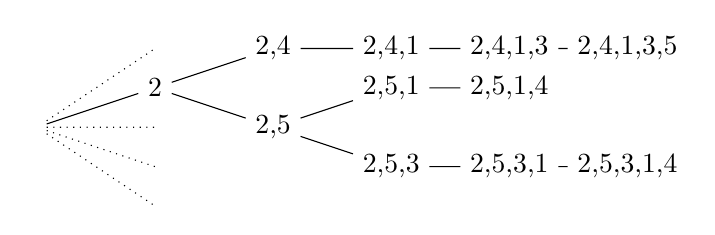
\begin{tikzpicture}[node distance=2cm]
\tikzstyle{level 1}=[sibling distance=0.5cm]
\tikzstyle{level 2}=[sibling distance=1cm]
	%    \tikzstyle{every node}=[draw]
    \node (root) {} [grow=right,dotted]
   	    child 
   	    child 
	    child 
    	child {node (2) {2} [black,solid]
	        child  {node (25) {2,5}
    	  		child {node (253)  {2,5,3}
    	  			child { node{2,5,3,1} child { node{2,5,3,1,4}} }
	      		}
    	   		child {node {2,5,1} child {node{2,5,1,4}}}        		        	          		        	  
	       	}
		    child {node {2,4}
		    	child {node {2,4,1}
		    		child {node {2,4,1,3} child {node {2,4,1,3,5} } }
		    	} 
		    }
	     }
	     child 
	 ;
%	\node at (253) {grid(1,1)};
\end{tikzpicture}
\caption{
Dette beslutningstræ viser backtracking når $2$ er valgt i række $1$. Blade i dybde $n$ angiver én løsning. Bemærk at roden er række 0.}
\label{fig:tree}
\end{center}
\end{figure}

%Jo højere oppe i træet vi fjerner et valg, jo større er det deltræ der vil blive fjernet.

\subsection{Bitmap-modellen}\label{bitmapmodellen}

\begin{figure}[!h]
\begin{center}
\begin{tabular}{|c|c|c|c|c|c}
\hline	0 & 0 & 0 & 1 & 0 \\
\hline	1 & 0 & 0 & 0 & 0 \\
\hline	0 & 0 & 1 & 0 & 0 \\
\hline	0 & 0 & 0 & 0 & 1 \\
\hline	0 & 1 & 0 & 0 & 0 \\
\hline
\end{tabular}
\end{center}
\caption{Samme eksempel som i figur \ref{fig:nq5eks}, men med en direkte binær repræsentation. En sat bit i en bitvektors position $i$ angiver en placering af en dronning i kolonne $i$.}
\label{fig:nq5eksbitmap}
\end{figure}

Idéen er beskrevet af \cite{Zongyan02} og implementeret af Takaken \ref{nqueenc}. Udover at repræsentere hver række på et skakbræt med en bitvektor, vedligeholdes for hver række  en bitvektor \textbf{bitmap} for de pladser, hvor det er muligt at placere en dronning.  Tilladte pladser begrænses af tidligere placeringer, så der bruges 3 bitvektorer til holde styr på optagede pladser, \textbf{horisontal}, \textbf{venstrediagonal}  og \textbf{højrediagonal}.

Efter hvert valg, hvor den valgte placering sættes i en bitvektor \textbf{bit}, udregnes de nye bitvektorer igen med følgende operationer. ($\gg og \ll$ angiver et logisk skift, således at der altid indføres et $0$ fra henholdsvis højre og venstre).
\begin{description}
	\item[horisontal] $down \lor bit$ 
	\item[venstrediagonal] $(venstrediagonal \lor bit) \ll 1$
	\item[højrediagonal] $(højrediagonal \lor bit) \gg  1$\footnote{Java bruger $>>>$ for logisk højre skift. For venstre er logisk og aritmetisk ækvivalent}
	\item[bitmap]	$bitmap = \lnot(venstre \lor horisontal \lor højre)$	
\end{description}


Da træets højde er begrænset af $n$, er det maksimale pladsforbrug $antal\ bits\ per\ bitvektor \times antal\ af\ bitvektorer \times n$. For at håndtere n op til 32, kan vi nøjes med 32 bits til at repræsentere en bitvektor. Pladsforbruget for $n=26$ er så $32\times 26 \times 4 = 3328\ bits$. Afhængig af implementationen og arkitekturens ordstørrelse vil dette variere. 

\subsection{Takakens optimeringer}\label{takalgo}

Mange løsninger er spejlinger og roteringer af andre - det totale antal løsninger kan afgøres ud fra antallet af unikke \emph{løsninger}. Ved kun at finde unikke løsninger, $S(n)$, og undgå de valg af placeringer der fører til løsninger som kan findes ved rotationer og spejlinger. Så kan vi fjerne store deltræer i vores beslutningstræ (se figur \ref{fig:tree}) og dermed mindske beregningstiden betragteligt.

I tabel \ref{tabel:unikkevstotale}, s.\pageref{tabel:unikkevstotale}, ses forskellen på antallet af unikke og totale løsninger. For hver løsning undersøges antallet af spejlinger og rotationer. \textbf{check()}-funktionen i Takakens implementation, afsnit \ref{nqueenc}, udfører dette. 
 
Der er forskellige måder at finde rotationer og spejlinger afhængig af dronninges placering i række 1. Optimeringerne er derfor delt op i to tilfælde

\begin{description}
	\item[Hjørnebræt] dronningen er i første række placeret i kolonne $1$.
	\item[Midterbræt] dronningen er i første række placeret i kolonnerne $2$  til og med $\lfloor n/2 \rfloor$.
\end{description}

Den første placering \footnote{For hjørnebræt er dette række 2, fordi den første dronning altid vil være placeret i hjørnet} af en dronning bestemmer hvilke valg vi kan undgå, og dermed mængden af det deltræ vi kan fjerne. Derfor vil der være forskel på andelen af løsninger som set på figur \ref{fig:midterandel}. Sammenholdt med figur \ref{fig:tidsvssol} kan vi se, forholdet mellem antallet af løsninger ca. angiver forholdet mellem beregningstiden bræt.

\begin{figure}
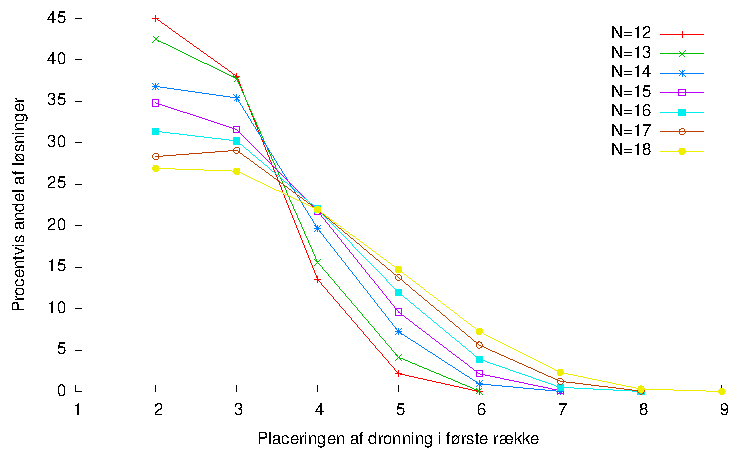
\includegraphics{../benchmarks/middleandel.pdf}
\caption{Bemærk at dette kun er \% af det totale antal løsninger for midterbræt. Det ses at antallet af løsninger falder drastisk for start-placeringer der nærmer sig midten.}
\label{fig:midterandel}
\end{figure}

\begin{figure}
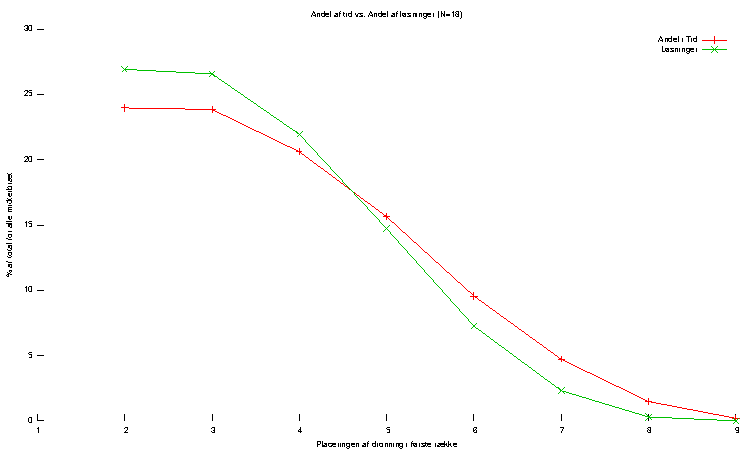
\includegraphics{../benchmarks/tidsandel.pdf}
\caption{Kørt for den iterative, fixme:caption}
\label{fig:tidsvssol}
\end{figure}

Det ses på figur/tabel FIXME at andelen af løsninger for bræt hvor den første dronning ikke placeres i et hjørne er over 90\% og stigende for større $n$, Det samme gælder for køretiden. Så hvis ca. 90\% af løsningerne findes i ét delproblem vil det også tage ca. 90\% af tiden at beregne dette delproblem. \fixme{flyt til benchmarks, og lav tabel der viser vi skal bare have at 90\% af køretiden er i middlebræt (og samme for køretiden??), jvnf. amdahls lov at vi ikke gider optimere hjørnebræt}

\subsection{Paralleliseringsmetode}\label{parallel}

Selve parallelisering er yderst simpel. Hvert delbræt kan løses uafhængigt efter at den første dronning er placeret. Antallet af løsninger for hvert bræt akkumuleres for at få det totale antal løsninger. Ved kun at forudvælge samme antal rækker, vil vi opnå en meget skæv fordeling af opgaver, jvf. figur \ref{fig:midterandel}. Dette problem er yderligere behandlet i afsnit \ref{opdelingipraksis}.

%Fordelingen af løsninger, når Takakens optimeringer ikke, er forskellig . Se \cite{etsi} side 7. 
%\fixme{Beskriv evt. med lidt matematik istedet.}. Det ses på figur \ref{fig:midterandel} og \ref{fig:tidsvssol}} at Takakens %%%optimeringer vil forandre denne både for antallet af løsninger og køretid. \fixme{rigtigt afsnit?)

\section{\mig\ og \oc}\label{migogoneclick}

	Her beskrives \mig\ og \oc\ overordnet. Afsnit \ref{mig} giver en introduktion til mulighederne i \mig. Afsnit \ref{oneclick} og \ref{begraensninger} beskriver muligheder for, og begrænsninger ifm. udvikling af \oc-applikationer. \mig\ er beskrevet i \cite{simplemig} og \cite{mig}, en introduktion til udvikling med \oc\ findes i 'Developer wiki' på \url{migrid.org}\footnote{Adgang kræver certifikat der kan bestilles på \url{https://mig-1.imada.sdu.dk/cgi-sid/requestcert_html.py}}.

\subsection{Minimum intrusion Grid}\label{mig}

\textsc{Minimum instrusion Grid}, herefter \mig, er et grid-system der sigter mod at stille så få krav for deltagelse som muligt - både overfor brugere og ressourcer. I \mig-terminologi er en ressource en enhed der kan sættes til at beregne et problem. Mange andre gridsystemer benytter ekstra software på den enkelte ressource, men undgår man helt dette, mindskes kompleksiteten af det samlede system dramatisk. 

\mig\ implementerer en model der sikrer fuldstændig anonymitet - det er umuligt for ressourcer at vide hvor de job de regner på kommer fra, og umuligt for brugere af vide hvor deres job afvikles. Få krav til deltagelse, anonymitet, sikkerhed\footnote{Baseret på ssl-certifikater} og skalerbarhed er hovedprincipperne bag \mig. Lige præcis til vores formål ligger der dog en begrænsning i den fuldstændige anonymitet. Vi er vi ude af stand til at parre specifikke job med specifikke ressourcer. En sådan mulighed kunne ellers danne basis for en alternativ løsning på scheduleringen af heterogene job, som beskrevet i afsnit \ref{opdelingogschedulering}. 
%\fixme{beskrivelse af anonymitet!, Det er vigtigt fordi det begrænser os, vi kan ikke vide noget om ressourcers hastighed, matche job til ressourcer(, osv?)}

%\fixme{Kort om sikkerhed i \mig}

%\fixme{kort om skalerbarhed i \mig}

\mig\ giver brugeren mulighed for at få adgang til et stort antal beregningsressourcer, uden at skulle bekymre sig om 
\begin{itemize}
	\item Hvor disse befinder sig.
	\item Hvem der ejer dem.
	\item Hvorvidt de hver især er istand til at løse den aktuelle opgave\footnote{Et givent problem kan f.eks. stille særlige krav til ressourcens arkitektur, eksisterende programmel, osv.}.
\end{itemize}
Her og i det nedenstående henviser udtrykket brugeren til en udvikler der ønsker at få beregnet et problem vha. \mig. 

Brugeren præsenteres for en abstraktion af \mig, der fremstiller et kendt paradigme fra unix-systemer; et hjemmekatalog hvori brugeren kan placere sine data- og programfiler. Brugerens interaktion med \mig\ foregår via en række scripts, der efterligner kendte kommandoer til manipulation af filer i hjemmekataloget, og introducerer kommandoer til at starte og stoppe job. Alt dette foregår over \emph{https}, som forespørgsler til en webserver. 

Interaktion med \mig\ kan alternativt foregå gennem et særligt webinterface. 
Begge metoder giver mulighed for at udføre følgende basale funktioner på \mig:
\begin{itemize}
	\item Igangsatte job.

	\item Se status på tidligere job.

	\item Få adgang til data-, program- og resultatfiler i hjemmekataloget. 
\end{itemize}

Et job sættes igang ved at køre kommandoen \emph{migsubmit} med en såkaldt mRSL-fil\footnote{\mig\ Resource Language} som argument. mRSL-filer indeholder beskrivelser af job der skal afvikles. Beskrivelsen fortæller \mig\ hvilken programfil der skal køres, med hvilke parametre, hvor lang tid jobbet forventes at tage og eventuelle krav jobbet har til de ressourcer der skal afvikle det. Et job har adgang til filerne i  hjemmekataloget. Resultatet af et job skrives til hjemmekataloget for senere at kunne aflæses af brugeren. For hvert job oprettes desuden 3 filer i hjemmekataloget. De indeholder hhv. exit-status, standard output og standard error, ganske som de kendes fra unix-systemer.

\mig\ tilbyder desuden at informere indsenderen via e-mail eller jabber\footnote{Open Source øjeblikkelig-besked-protokol, se mere på \url{http://www.jabber.org}} når et job afsluttet. 

\subsection{\oc} \label{oneclick}
\oc\ er en java-applet der muligør deltagelse i \mig, uden andre forudsætninger end en webbrowser og java. Tilgengæld er denne metode begrænset til at afvikle programmer, der er tilgængelige som java-bytekode. Brug af \oc\ giver adgang til et enormt (potentielt) antal beregningsressourcer, da det gør det muligt for ganske alm. mennesker at bidrage regnekraft til gridet.

Implementerer man sit problem i en \oc-applet vil det kunne afvikles på alle \oc-ressourcer, uden at skulle specificere særlige krav til arkitektur med videre. Til gengæld vil det være begrænset til kun at køre på \oc-ressourcer.
\oc\ er især interessant i forbindelse med hvad man kunne kalde sociale beregninger, det vil sige beregningsprojekter som almindelige mennesker kunne have interesse i at bidrage til, eller endog konkurrere om at bidrage mest til. Kendte eksempler på sådanne projekter er SETI@home (BOINC) og FOLDING@home. Til forskel fra disse, sammenlignelige projekter, er \oc\ ikke applikationsspecifikt. \oc-udviklere kan implementere nye projekter og få dem kørt, uden at der skal foretages nogen ændringer på ressourcesiden. Alt hvad der er specifikt for applikationen sendes med jobbet til \oc-ressourcen. Omvendt kan en \oc-ressource ikke bestemme hvilke job-typer den vil afvikle eller hvilke projekter den vil deltage i.

\oc\ indeholder java-klasser til læsning og skrivning af filer i hjemmekataloget på \mig\, samt checkpointing af det kørende job. 

\subsubsection{Checkpointing}
\oc\ indeholder kode til oprettelse af checkpoints under kørslen af et job. Et checkpoint er en gemt programtilstand, hvorfra det er muligt at fortsætte afviklingen. \oc\ indeholder desuden mekanismer til genetablering af programtilstanden fra et givent checkpoint. Når et \oc-job sendes til en ressource, sendes det nyeste checkpoint med, hvis et sådant eksisterer. \oc\ sørger så for at genetablere tilstanden før eksekveringen af jobbet starter. Dette er præcis den funktionalitet vi behøver for at kunne sikre, at vi ikke skal køre en beregning forfra, når en ressource forlader gridet.
Checkpoint foretages ved at serialisere det kørende job-objekt\footnote{\mig-applettens hoved objekt, der nedarver fra MiGJob-klassen} til hjemmekataloget på \mig. Det er altså kun objekt-grafen, med rod i MigJob-objektet, og eventuelle åbne filer, der overlever på tværs af et checkpoint. Hverken kald-stak eller programtæller overlever.

\subsubsection{\oc-specifikke begrænsninger}\label{begraensninger}
En java-applet afvikles i et lukket miljø, en såkaldt sandkasse, for at beskytte den maskine der afvikler appletten. En applet skal desuden overholde \texttt{Applet security model}\footnote{\url{http://java.sun.com/sfaq/}}. Dette giver en række begrænsinger vi bliver nødt til at forholde os til
\begin{itemize}
	\item Appletten kan maksimalt allokere 64MB hukommelse.
	\item Java's JNI (Java Native Interfaces) kan ikke benyttes fra appletter. 
	\item Ingen adgang til at læse/skrive lokale filer.
	\item Appletten er begrænset til kun at kunne oprette netværksforbindelser til den ip-adresse den er hentet fra.
\end{itemize}

Det bliver naturligvis et krav at alle delproblemer vi sender ud kan beregnes uden at bruge mere end 64MB hukommelse på klienten. Uden JNI har vi ikke mulighed for måle cputid.

\section{Problemstørrelse og jobschedulering}\label{opdelingogschedulering}

\begin{figure}[!h]\label{fig:spildtidventetid}
\begin{center}

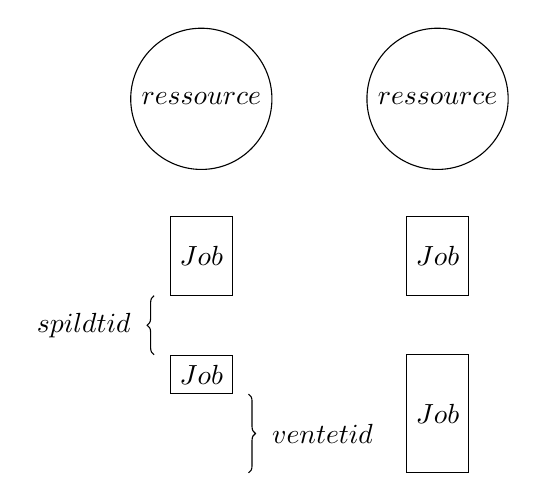
\begin{tikzpicture}%[show background grid]
%\tikzstyle{background grid}=[draw, black!50,step=.5cm]


\draw[snake=brace] (-0.6,-3.25) --
        node [draw=none,left=0.5em,fill=none]{$spildtid$}(-0.6,-2.5) ;
\draw[snake=brace] (0.6,-3.75) --
        node [draw=none,right=0.5em,fill=none]{$ventetid$}(0.6,-4.75) ;

\tikzstyle{every node} = [draw]
\begin{scope}
\path (0,0) node[circle] {$ressource$};
\path (0,-2) node[rectangle,minimum height=1cm] {$Job$};
\path (0,-3.5) node[rectangle] {$Job$};
\end{scope}
%\draw[fill,gray] (0,-3.5) circle (1.5pt);
%\draw[fill,gray] (0,-3.66666) circle (1.5pt);
%\draw[fill,gray] (0,-3.83333) circle (1.5pt);

\begin{scope}
\path (3,-0) node[circle] {$ressource$};
\path (3,-2) node[rectangle,minimum height=1cm] {$Job$};
\path (3,-4) node[rectangle,minimum height=1.5cm] {$Job$};
\end{scope}        
%\draw[thick,dashed,<->] (4,-4) -- (4,-1);

\end{tikzpicture}		
\caption{Illustration af \emph{spildtid} og \emph{ventetid}. Tegningen viser afviklingen af et samlet problem med 4 delproblemer, kørt på 2 ressourcer.}


\end{center}
\end{figure}


%Figur over summen
\begin{figure}[!h]
\begin{center}

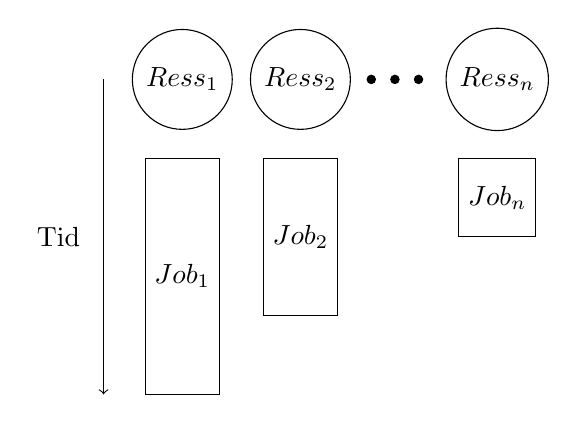
\begin{tikzpicture}%[show background grid]
\tikzstyle{background grid}=[draw, black!50,step=.5cm]
\tikzstyle{every node} = [draw]

\draw[->] (0,0) -- node[draw=none,left=0.5em]{Tid} (0,-4);

\draw (1,0) node[circle] {$Ress_1$};
\draw (2.5,0) node[circle] {$Ress_2$};
\draw[fill] (3.4,0) circle (1.5pt);
\draw[fill] (3.7,0) circle (1.5pt);
\draw[fill] (4.0,0) circle (1.5pt);
\draw (5,0) node[circle] {$Ress_n$};

\path (1,-2.5) node[rectangle,minimum height=3cm] {$Job_1$};
\path (2.5,-2) node[rectangle,minimum height=2cm] {$Job_2$};
\path (5,-1.5) node[rectangle,minimum height=1cm] {$Job_n$};

\end{tikzpicture}		
\caption{Illustrerer en tænkt opstilling hvor \texttt{\#Ress=\#Job}} 
\end{center}
\end{figure}

%Square beregningstid
\begin{figure}[!h]
\begin{center}

\begin{tikzpicture}%[show background grid]
\tikzstyle{background grid}=[draw, black!50,step=.5cm]
\tikzstyle{every node} = [draw]


\draw (0,0) node[rectangle,minimum height=3cm,minimum width=3cm] {$T_1$};
\draw (-0.75,-0.75) node[rectangle,minimum height=1.5cm,minimum width=1.5cm] {$T_2$};

\draw[->] (-1.25,-1.75) -- node[draw=none,below=0.5em]{$\frac{1}{Hastighed}$} (2,-1.75);
\draw[->] (-1.75,-1.25) -- node[draw=none,left=0.5em]{Jobstørrelse} (-1.75,2);

\end{tikzpicture}		
\caption{Illustration af at både ressourcehastighed og jobstørrelse variere. Arealet er beregningstiden. Bemærk at beregningstiden stiger med faldende ressourcehastighed}\label{fig:lillekassestorkasse} 
\end{center}
\end{figure}


I det følgende benyttes disse forkortelser for ofte anvendte begreber.
\begin{description}
	\item[$T$] Beregningstiden for én opgaver på én ressource.  
	\item[\texttt{\#Job}] Antallet af job.
	\item[\texttt{\#Ress}] Antallet af ressourcer.  
\end{description}

Desuden defineres \emph{spildtid} som den tid en ressource benytter til at sende resultater og hente nye job. Denne tid kan spares hvis jobbets beregningstid svarede til den tid ressourcen er tilgængelig. Omvendt defineres \emph{ventetid} som den tid en ressource ikke benyttes, fordi der ikke er job klar til beregning. Disse tider er illustreret på figur \ref{fig:spildtidventetid}.

Et centralt emne ved parallelisering af algoritmer er partitionering af de data der beregnes på. Vi kan forestille os en ideel situation, hvor:
\begin{enumerate}
	\item Job er homogene. \label{beregningstid}
	\item $\texttt{\#Job}$ er præcis lig $\texttt{\#Ress}$.\label{antal}
	\item Ressourcer er homogene. 
	\item Ressourcer er permanente.
	\item Repræsentationen af job og resultater har minimal størrelse.\label{jobbeskrivelse}
\end{enumerate}

I denne, ideelle situation, opnås maksimal udnyttelse af tilgængelige ressourcer - der er ingen \emph{ventetid}. Samtidig minimeres \emph{spildtiden} i forbindelse med jobskift og dataoverførsel.
 
Som beskrevet i afsnit \ref{takalgo}, stiger beregningstiden for et delproblem med antallet af løsninger i delproblemet. Vi kan altså ikke, ved opdeling af problemet, kende de enkelte delproblemers beregningstid. I stedet kan vi opdele problemet i dele med samme data-størrelse - hvilket i praksis vil sige at samme antal dronninger mangler at blive placeret. 

Beregningstiden kompliceres yderligere af at delproblemerne skal beregnes på heterogene ressourcer, som vi ikke kan kende hastigheden af før delopgaven er færdigregnet. Heller ikke $\texttt{\#Ress}$ har vi mulighed for at kende. 

Den reelle situation er altså langt fra den ovennævnte ideelle. Problemet bliver at finde den opdeling af job der bringer beregningstiden nærmest den fra den ideelle situation, og at gøre dette indenfor følgende rammer:
\begin{itemize}
	\item Ressourcer er heterogene.
	\item Ressourcer er upålidelige.
	\item $\texttt{\#Ress}$ varierer.
	\item Job er heterogene.
\end{itemize}

Idet både ressourcer og job er heterogene kan de ses som et samlet problem, blot af en anden størrelsesorden. Figur \ref{fig:lillekassestorkasse} illustrerer hvor hurtigt beregningstiden vokser.
Da der arbejdes med heterogene ressourcer kan den minimale \emph{spildtid} ikke opnås. 
Antager man at $\texttt{\#Ress}$ er fast vil det mindst mulige, samlede \emph{spildtid} opnås ved at have $\texttt{\#Job} = \texttt{\#Ress}$. \emph{ventetiden} vil til gengæld være stor. 

\emph{Ventetiden} vil være summen af forskellene i beregningstider op til den langsommeste ressource, for alle ressourcer.   
 
\begin{displaymath}
	\sum_{i=1}^{\texttt{\#Ress}} T_{max} - T_{i} 
\end{displaymath}

Antager man igen at $\texttt{\#Ress}$ er fast, vil man, med en jobmængde der er større end ressourcemængden, få en mere jævn udnyttelse af ressourcerne. Jo større $\texttt{\#Job}$ i forhold til $\texttt{\#Ress}$, des mere jævnt bliver ressourcerne brugt, og des mindre bliver den sammenlagte \emph{ventetid}. Dette er netop fordi den jobstørrelsen falder når antallet af job stiger. 

Når $\texttt{\#Job} > \texttt{\#Ress}$ vil det værste tilfælde for \emph{ventetid} opstår, når der kun er et job tilbage at beregne, og dette job netop er det største. I dette tilfælde vil \emph{ventetiden} mindst være 
\[
T_{max} \times \#Ress -1
\]
.



%Er den maksimale forskel i hastighed, $maxdif_{h} = Hast_{r}$ - $Hast_{q}$, mellem to vilkårlige ressourcer $r$ og $q$, og den maksimale forskel i beregningsstørrelse $maxdif_{str} = Str_{j}$ - $Str_{k}$ mellem to job $j$ og $k$, 
Jo mere homogene vores job er, des bedre kan vi tilpasse \texttt{\#Job} så vi minimerer både \emph{vente}- og \emph{spildtid}. 

Uanset jobstørrelser, er det essentielle, at undgå ubenyttede ressourcer, uden at komme til at skrue for meget op for antallet af job, og derved øge \emph{ventetiden}.

%\fixme{Beregning af spildtid skal være summation. "Beregningerne" skal generelt gøres klarere. Husk at ressourcehastighed ikke længere er i tid. Brug havelåge til at markere antal.}

%\fixme{Vi skal have en tegning af nogle ressourcer og de job de kører/har kørt. Hvor vi kan markere de forskellige tidsbegreber. Spildtid ændres til ventetid. Overhead ændres til spildtid.}


\section{Opdeling af opgaver i praksis}\label{opdelingipraksis}
	Herunder vil vi, fortrinsvis ved at kigge på data for problemstørrelser for mindre $n$, forsøge at finde frem til en optimal opdeling af problemet for $n=26$.

I \mig\ skemalægges afviklingen af job som en FIFO-kø. Dvs. at job afvikles i samme rækkefølge som de submittes til gridet. Ved afbryding af jobbet eller ved udløb af tidsfristen for afvikling af jobbet placeres jobbet bagerst i køen. 

Den løsning der er implementeret, i forbindelse med denne opgave, kan bedst karakteriseres som såkaldt \emph{statisk orkestration}. I det opdelingen i delproblemer er endeligt foretaget inden beregningen af delproblemer begynder. Som beskrevet i afsnit \ref{opdelingogschedulering} er der et grundlæggende problem ved en statisk opdeling, nemlig at beregningen ikke kan tilpasse sig til en forøgelse af mængden af ressourcer. I stedet bliver man nødt til fra starten at generere nok opgaver til at kunne udnytte en eventuel ressourcetilgang. Samme problem opstår, på grund af heterogene ressourcer og opgaver, når antallet af delopgaver falder henimod slutningen af udregningen. 

For at afhjælpe dette problem kan joboprettelsen gøres mere dynamisk. Den indledende mængde delopgaver kan tilpasses det øjeblikkelige antal ressourcer. Herefter opdeles en eller flere af disse i mindre delopgaver, så snart der er ledige ressourcer. På denne måde sikres det at ingen beregningskraft står ubrugt hen. 
Det bedste valg af job til genopdeling vil være det der kræver mest beregningstid, da dette vil resultere i den mindst mulige spredning i beregningsstørrelse for alle opgaver efter opdelingen\footnote{Idet alle nye opgaver vil være mindre end det oprindelige, men ingen vil være mindre end den mindste der blev oprettes, hvis vi valgte en anden end den største til opdeling.}. På figur \ref{fig:tidsvssol} ser vi eksempler for beregningstiden for hver delopgave. Det er tydeligt at de følger et mønster, og at vi kan bestemme et indbyrdes størrelsesforhold mellem alle midterbræt. Dette giver os en god idé om hvilken delopgave det bedst kan betale sig at splitte op. Tilgengæld har vi ikke mulighed for at vide, om beregningen af denne opgave allerede er ved at være færdig, og en opsplitning ville være uhensigtsmæssig. 

Alternativet til den dynamiske joboprettelse er en statisk, hvor spredningen af beregningsstørrelser for delproblemer forsøges minimeret ud fra antagelser om fordelingen af løsninger i delproblemerne. Disse antagelser kan vi kun retfærdiggøre ud fra vores viden om fordelingen for mindre $n$. Det er altså den samme viden om fordelinger vi gør brug af her, som i den dynamiske model. Her opdeler vi blot de (formodet) mest beregningstunge problemer fra starten. Vi sparer altså overvågning af projektet, men foretager til gengæld opdelinger før vi er sikre på at vi har det overskud af ressourcer, der gør dem fordelagtige.    

\fixme{Fixed? Beskriv den anden mulighed : at gøre job-genereringen mere intelligent, så vi kan være sikre på at få job der ikke har ligeså forskellige størrelser.}

\fixme{hvad kan vi sige om om beregningstiden for problemer med samme data-størrelse? Øvre grænse for variationen i køretid? Indsæt reference til benchmarks, der viser beregningstid for hvert delproblem, og skriv noget om hvad benchmarks viser vi kan regne med ifm. beregningstid}


\section{Resultathåndtering}\label{resultatindsamling}
\subsection{Indsamling og visning}
En måde et holde styr på den samlede beregning af en løsning på \nq\ er, at have en vedligeholdelsesproces kørende, der sørger for at 
\begin{itemize}
	\item Genkøre fejlede job.
	\item Indsamle resultater fra færdige job.
	\item Muliggøre løbende projektstatus og offentliggørelse af resultater. 
\end{itemize}
Dette program kan for eksempel være det samme, der står for at oprette vores job i første omgang. 

En enkel metode kunne være at lade \mig\ sende e-mail når job er færdige, og så sætte .procmail el.lign op til automatisk at kalde et script der henter status/stdout/stderr filer og hive resultater ud og lægge sammen når der
kommer en mail.

Yderligere kunne det være interessant at have mulighed for at tilpasse ikke-kørte job på baggrund af informationer om gridets tilstand (antallet af tilgængelige ressourcer). Dette er en praktisk måde at implementere den dynamiske joboprettelse der beskrives i afsnit \ref{opdelingipraksis}. 

\subsection{Verifikation}
Da der, på nuværende tidspunkt, ikke er nogen form for pointsystem i \mig/\oc,
er der ikke den store chance for folk vil prøve at snyde for at være den der
laver flest point. Hvis folk derfor sender forkerte resultater ind må det
nærmere betegnes som sabotage, og ikke snyd. Måder man kan forhindre
snyd/sabotage kan være at sende de samme job ud flere gange, og sammenligne
resultater, eller foretage stikprøve kontrol hvor man selv regner nogle af
jobbene ud og sammenligner resultatet. 

\subsection{Resultatets størrelse}
For at sikre at vi ikke får overløb ved brug 64-bit tokomplement heltal, undersøges udviklingen af resultaterne for lavere n.
På figur \ref{figur:maxantal} ses det at den maximale positive værdi for \texttt{long} er en faktor \~1000-500  større end løsningen for n=25. Samtidig viser figur \ref{figur:loesningfaktor}, at man kan formode resultatet for $n=26$ er ~10 gange større end for $n=25$. Denne forskel vurderes signifikant nok til at vi kan regne n=26 ud for 64-bit tokomplement heltal.

\begin{figure}[h!]
\begin{center}
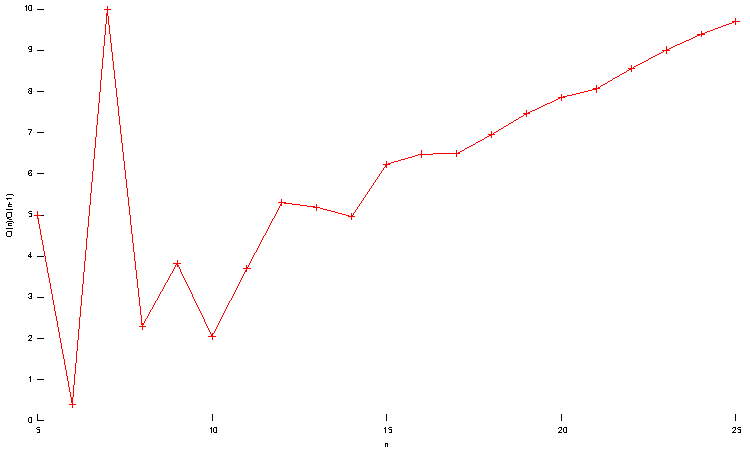
\includegraphics{../benchmarks/resultatstorrelse.pdf}
\caption{Figuren viser $Q(n)/Q(n-1)$ for $n=15\ldots25$. Der ses faktor som stabiliseres og er let stigende. $n=26$ kan altså formodes at være ca. 26 gange større}
\label{figur:loesningfaktor}
\end{center}
\end{figure}

\begin{figure}[h!]
\begin{center}
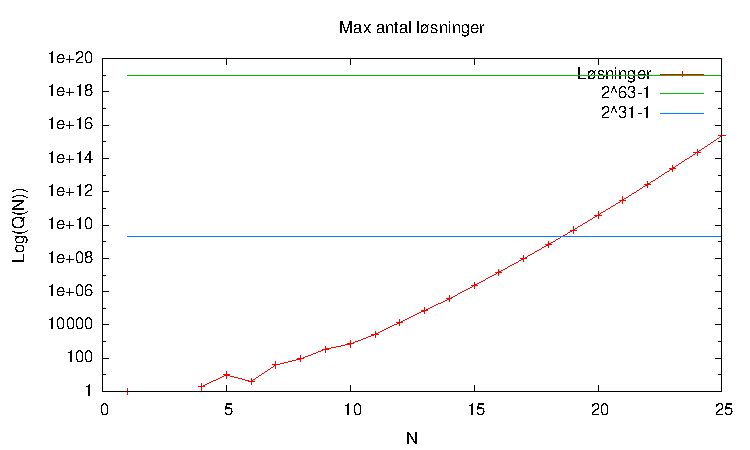
\includegraphics{../benchmarks/maxantal.pdf}
\caption{Viser antallet af løsninger på en logaritmisk skala. Derudover er Java's \texttt{long} og \texttt{int} maximale positive værdi inkluderet. Det ses at løsningen for Q(25) er ca. en faktor 400 mindre end \texttt{long} i Java.}
\label{figur:maxantal}
\end{center}
\end{figure}



\section{Beskrivelse af implementeringen}\label{implementering}
\begin{verse}
	Følgende er ment som en beskrivelse af, og læsevejledning til programmets kildekode, såvel som en vejledning til afvikling af programmet med forskellige formål. 
\end{verse}

Den udviklede kildekode er beregnet til at undersøge hvordan \nq\ paralleliseres. Hovedformålet er at kunne afvikle prøvekørsler, der vil give en forståelse af den optimale jobopdeling- og scheduleringsstruktur for $n=26$.

Kildekoden implementerer en rekursiv og en iterativ udgave af Takakens algoritme, som beskrevet i afsnit \ref{takalgo}, og giver mulighed for enten at afvikle disse lokalt eller indsende dem som job til \mig. Den lokale afvikling er så vidt muligt den samme kode som hvad der afvikles i \oc. Dette er med henblik på at sikre korrekthed og kunne foretage flest mulige test lokalt, før de køres på gridet. 


Den udviklede kildekode er organiseret i følgende filer:

\begin{description}
	\item[NQueenBoards.java] jobgeneratoren, parallel-nqueen-algoritme, der genererer delproblemer i form af boards, hvor de første $m$ dronninger allerede er placeret. 
	\item[Board2.java] Basis-klasse for wrapper-klasser til backtrack
	\item[CornerBoard.java] klasse til backtrack for cornerboards
	\item[MiddleBoard.java] lasse til backtrack for middleboard
	\item[CheckPointer.java] implementerer checkpointing
	\item[CheckPointActionMiG.java] implementerer checkpointing
	\item[NQueenJob.java] hovedklassen for et \mig-\oc-job. 
	\item[MiGSSLSocketFactory.java] hjælpeklasse til MiGClient-klassen
	\item[MiGClient.java] java-implementation af en del af \mig-hjælpeprogrammerne
	\item[MiGJob.java] klasse der beskriver et job og kan generere en .mRSL-fil
	\item[CornerBoardBoardTest.java] unittests til CornerBoard
	\item[MiddelBoardTest.java] unittests til MiddleBoard
	\item[NQueens.java] Testfil - Direkte java-port af Takakens c-kode. Kan køres som \oc\ job.
	\item[NQueensL.java] Testfil - Direkte java-port af Takakens c-kode. Kan køres lokalt.
	\item[Board.java] Testfil - Hjælpeklasse til NQueens/NQueensL
	\item[Globals.java] Testfil - Hjælpeklasse til NQueens/NQueensL
\end{description}

\subsection{NQueenBoards.java}

NQueenBoards er hovedklassen, omend det er begrænset hvor meget der egentlig
bliver gjort i den. Den opretter et nyt CornerBoard objekt (se
\ref{cornerboard}) og et nyt MiddleBoard objekt (se \ref{middleboard})
kører deres init metode og tilføjer outputtet herfra blivet stoppet på en hægtet
liste. 
herefter bliver iterateOneLine kørt \texttt{maxSteps} gange

\texttt{maxSteps} er en variabel man kan skrue på for at
ændre antallet af boards der bliver genereret. Den angiver mange dronninger vi
forud placerer på vores bræt. Det skal dog bemærkes at der er forskel på hvor
mange bræt MiddleBoard og CornerBoard genererer ud fra \texttt{maxSteps}, der
bliver genereret flere CornerBoards, da der allerede fra start er placeret en
dronning i hjørnet.

På nuværende tidspunkt er der en lille mængde manuelt arbejde i det. Som det ser
ud for øjeblikket er der 2 muligheder i NQueenBoards, som også kan kombineres. 
Man kan vælge at submitte jobbene direkte (P.t. er denne funktion dog lavet om
til at gemme zip filen lokalt da MiG ikke er glad for at submit and extracte en
zip fil med over 12000 job). Man kan også få NQueenBoards til at beregne
resultatet (kun en god ide for ikke alt for store værdier af $n$). Disse 2
muligheder vælger man ved at ud/indkommentere henholdsvis linje 73-74 og linje
83-96 

\subsection{Board2}

Board2 er en abstract klasse der, hvor diverse funktionalitet, der er fælles for
Corner- og MiddleBoard er implementeret.

\subsection{CornerBoard.java}
\label{impcornerboard}

CornerBoard er egentlig et andet, og måske lidt mere sigende navn, end
Backtrack1 fra \ref{nqueensc}. De 2 vigtigste dele af denne klasse er
backtrackRecursive og backtrackIterative. backtrackRecursive er den samme som
Backtrack1 fra den oprindelige c-kode. Da vi gerne vil have mulighed for at lave
checkpoints, er der blevet lavet en iterativ udgave af backtrackRecursive, dette
skyldes at checkpoint ikke gemmer kaldstak og programtæller, så vi ville ikke
kunne starte op fra et checkpoint med backtrackRecursive. \fixme{beskrivelse af
iterativ udgave}

\subsection{MiddleBoard.java}

I samme stil som CornerBoard, er MiddleBoard tilsvarende Backtrack2 fra
\ref{nqueens}. Her har vi igen en backtrackRecursive og backtrackIterative, hvor
backtrackRecursive er den samme som Backtrack2 fra \ref{nqueens} og
backtrackIterative er ændret således at vi kan lave checkpoints.

\subsection{NQueenJob}

NQueenJob i sig selv laver ikke så meget, den indlæser et serialiseret objekt
enten det der er specificeret som argument, eller det som er blevet checkpointet
tidligere. Herefter ser den efter om objektet gerne vil have at der laves
checkpoints, og i så fald starter checkpointing. Derefter kalder den objektets
backtrack() metode. Når beregningen er færdig stopper den checkpointing og
skriver resultatet til stdout.

\subsection{CheckPointer.java, CheckPointActionMiG.java}

\fixme{Beskrivelse af hvordan vi checkpointer og de lokale tests af checkpoint}
Disse 2 klasser bliver brugt til at lave checkpoints. Hovedideen bag vores
checkpointing er at vi venter i 15 min, derefter siger vi så at nu er vi klar
til at lave checkpoint, og når backtrackIterative så kommer til et sted hvor den
kan lave checkpoint, gør den dette og bagefter fortsætter den så, mens vi venter
endnu 15 min. osv. osv. 

\subsection{NQueens, NQueensL, Board, Globals}

Disse kildekode filer indeholder vores først "port" af Takakens kode til java,
og er så vidt muligt en copy/paste af Takakens kode, og er derfor ikke særlig
interessante. 

\subsection{MiGClient, MiGJob, MiGSSLSocketFactory}

Disse klasser er lavet for at kunne lave \mig-job og submitte dem direkte uden
at manuelt skulle køre migput/migsubmit. Den ville eventuelt kunne udvides til
også at foretage overvågning/resultatopsamling af \mig-kørsler.

\subsection{CornerBoardTest, MiddleBoardTest}

Disse to klasser er lavet for nemt at kunne teste CornerBoard og MiddleBoard
hver gang der var blevet lavet ændringer i dem. 

\subsection{Problemer med implementeringen}

Så vidt vi har kunnet se, rydder \mig ikke op i checkpoints, og sletter de
gamle. Dette ville måske kunne skabe problemer. Et checkpoint fylder for os omk
1.7Kb. Pt. laver vi et checkpoint hvert kvarter. Hvis man regner med at
løsningen for $n=26$ vil tage omk 26 gange så langt tid at finde som for $n=25$
bliver dette i sidste ende til omkring 80Gb. Ydermere, hvis man har mange
ressourcer kørende parallelt ville der hurtigt kunne blive akkumuleret en masse
checkpoints. 

Et andet problem med vores implementation er at den regner forkert når
$maxSteps>n/2$. Vi har ikke umiddelbart fundet en forklaring på hvorfor, men da
vi ikke vil komme op på en $maxSteps$ større end 3 måske 4 for $n=26$ har vi
ikke kigget yderligere på det.

\subsection{Optimeringer af java-koden}
Før den endelige kørsel for $n=26$ bør følgende optimeringer foretages:

\begin{description}
	\item[Serialiserede objekter erstattes af argumenter]
	De serialiserede \texttt{Board}-objekter var en nem måde at få oprette opgaver på en måde der både kunne bruges på i \oc\ og til lokale tests. Brugte vi istedet blot parametre direkte i \texttt{mRSL}-filen ville vi spare en masse overførselstid. Både ved indsendelse af job og ved jobskift på ressourcerne.  
	\item[Al brug af \texttt{Array} undgåes]
	Vi benytter en række \texttt{Array}s til at simulere en stak for de oprindelige argumenter til \texttt{backtrack}. Enhver tilgang til et \texttt{Array} betyder i java at der fortages en \texttt{BoundsCheck}. Brugte vi i stedet en f.eks. en hægtet liste ville vi kunne undgå dette.
	 
\end{description}


\fixme{Skriv derefter uddybende til de øverste.}




\section{Afprøvning og benchmarking}\label{benchmarks}

%Benchmarking-delens fremmeste formål er at finde svar på en række spørgsmål inden udregningen sættes igang.
%Reelt har vi kun en enkelt parameter vi kan skrue på, nemlig $m$ - antallet af dronninger vi placerer på hver board før vi genererer et \mig\ job til at regne videre på det board. te
%Hvilket forhold mellem 

%\subsection{Takaken}
%\subsection{Java port}
%\subsection{Java port v2}
%\subsubsection{Rekursion vs. Iterativ metode}
%\subsubsection{Iterativ med checkpoints}
%\subsection{MiGrid}

Benchmarking-delens fremmeste formål er at finde svar på en række spørgsmål
inden udregningen sættes igang.  Reelt har vi kun en enkelt parameter vi kan
skrue på, nemlig $m$ - antallet af dronninger vi placerer på hver board før vi
genererer et mig job til at regne videre på det board.  Hvilket forhold mellem 
\fixme{what?}
%\subsection{Takaken}
%\subsection{Java port}
%\subsection{Java port v2}
%\subsubsection{Rekursion vs. Iterativ metode}
%\subsubsection{Iterativ med checkpoints}
%\subsection{MiGrid}

\subsection{Lokale tests}

Vi starter med at teste de forskellige udgaver af koden lokalt, så vi har en
baseline at sammenligne med.

Alle lokale tests er kørt på en IBM T43, med en pentium m 1.86Ghz cpu, 

Java koden er kompilet med javac

\begin{verbatim}
alex@roadrunner:~/temp/queens/src/main/java$ javac -version
javac 1.5.0_11
\end{verbatim}

C koden er kompilet med \texttt{gcc -Os -O2 -o nq nqueens.c}

\begin{verbatim}
alex@roadrunner:~/temp/queens/src/main/java$ gcc --version
gcc (GCC) 4.1.2 (Ubuntu 4.1.2-0ubuntu4)
\end{verbatim}

De første tests er kørt på revision 77 (i forbindelse med den iterative test er
udskrivning af debug info til skærmen dog blevet kommenteret ud)

\begin{figure}[h]
\begin{center}
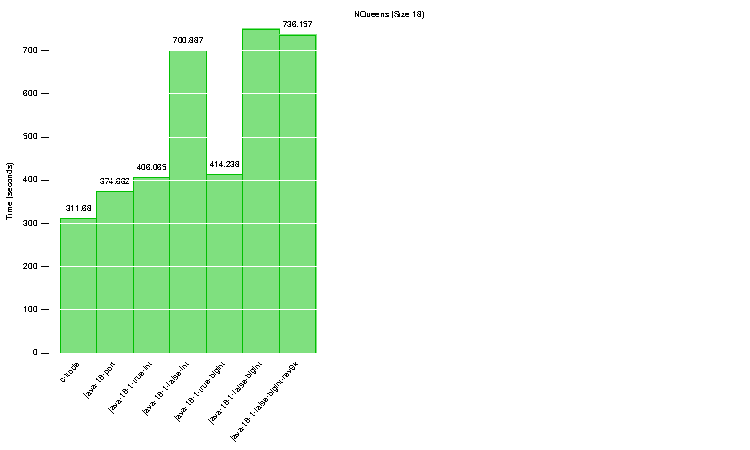
\includegraphics{../benchmarks/lokal.pdf}
\caption{insert proper caption here } 
\label{figur:lokal}
\end{center}
\end{figure}
\fixme{caption, or no caption.. this graph is redundant information}

Som det ses er C udgaven en smule hurtigere end den direkte java port, der igen
er lidt hurtigere end den paralleliserede udgave af koden, når den kører
rekursivt. Den iterative udgave er væsentlig langsommere..

Den parallelle udgave af koden er i dette tilfælde her kørt med
\texttt{maxSteps} på 1. 
\begin{figure}[h]
\begin{center}
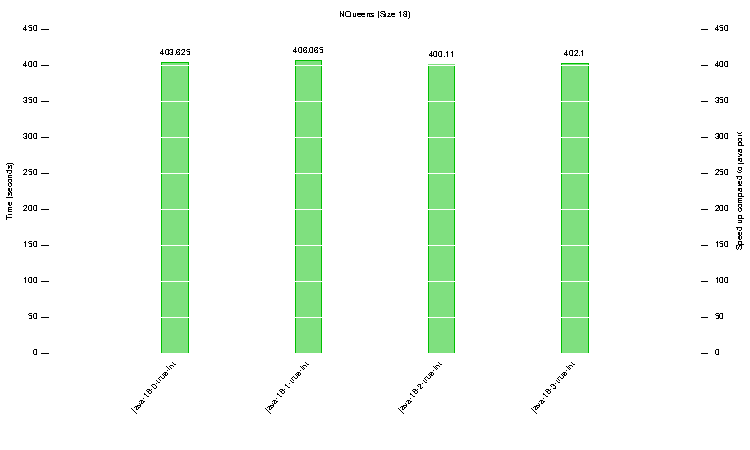
\includegraphics{../benchmarks/maxsteps.pdf}
\caption{insert proper caption here } 
\label{figur:maxsteps}
\end{center}
\end{figure}

På figur \ref{figur:maxsteps} er vidst kørsler for $n=18$ for forskellige
$maxSteps$. 
Som det ses, har det ikke den store indflydelse på performance hvor stor
$maxSteps$ er, der er altså ikke det store overhead ved at generere en masse
opgaver og løse dem bagefter, når det kører lokalt. 

Det skal også nævnes at for $maxSteps>n/2$ vil vores program regne forkert.
Dette skyldes \fixme{ja.. hvad skyldes det.. }


I tabel \ref{tabel:noboards} kan det ses hvor mange boards der bliver genereret
for forskellige $n$ og $maxSteps$. 

\fixme{hvor mange jobs bliver der lavet for de forskellige maxsteps, indsæt
tabel?}
\begin{table}
	\begin{center}
		\begin{tabular}{|c|c|c|c|c|c|}
			\hline N  & maxSteps  & boards & n  & maxSteps & boards \\
			\hline 15 & 0         & 18     & 17 & 0        & 21     \\
			\hline 15 & 1         & 173    & 17 & 1        & 243    \\
			\hline 15 & 2         & 1310   & 17 & 2        & 2282   \\ 
			\hline 15 & 3         & 8349   & 17 & 3        & 18161  \\
			\hline 15 & 4         & 43961  & 18 & 0        & 23     \\
			\hline 16 & 0         & 20     & 18 & 1        & 289    \\
			\hline 16 & 1         & 212    & 18 & 2        & 2983   \\
			\hline 16 & 2         & 1797   & 18 & 3        & 26204  \\
			\hline 16 & 3         & 12840  &    &          &        \\
			\hline 16 & 4         & 76224  &    &          &        \\
			\hline
		\end{tabular}
		\caption{Antal Boards der bliver genereret}
		\label{tabel:noboards}
	\end{center}
\end{table}

Alle tests er i første omgang kørt 5 gange, dette blev gjort for at se om
køretiden svingede meget, da dette ikke lader til at være tilfældet (se figur
\ref{figur:b1} vil resten af testene kun blive kørt 1 gang.. 

\begin{figure}[h]
\begin{center}
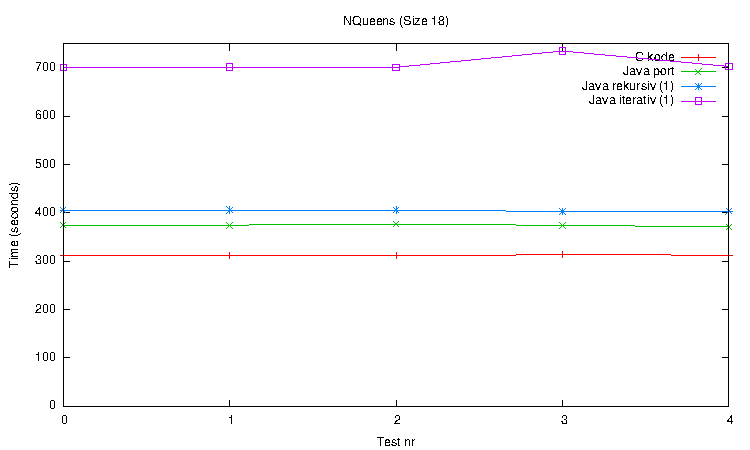
\includegraphics{../benchmarks/b1.pdf}
\caption{insert proper caption here } 
\label{figur:b1}
\end{center}
\end{figure}

Nu skal vi så se på hvor hurtigt det kører når vi smider det efter MiGrid. 
Disse tests er kørt med \texttt{maxSteps} 0 og 1.

\fixme{indsaet en graf, eller bare resultaterne og henvis til b3?}
De foregående tests er kørt med kode der bruger \texttt{int} til at gemme resultaterne,
i de næste tests er \texttt{int} skiftet ud med \texttt{BigInteger} (revision
83
\clearpage
Sammenligning af alle benchmarks

Som det ses på figur \ref{figur:lokal} kører den iterative udgave af koden fra
rev. 83 (med bigint) utroligt langsomt i forhold til foregående udgaver.  Dette
skyldes en en linje kode, der ikke var blevet kommenteret ud. Denne linje
konkatenerede to strenge. Uden denne linje kører koden væsentlig hurtigere, som
det kan ses på den sidste søjle i figur \ref{figur:lokal}


Som det kan ses på figur \ref{figur:lokal} kører den rekursive kode en smule
langsommere med \texttt{BigInteger} end med \texttt{int}, hvor tiden stiger fra
406.xxx til 414.xxx\fixme{indsaet rigtige tal}, hvilket svarer til en forøgelse
på knap 2\%

\subsection{overhead ved jobskifte}

I MiG\_main() metoden i NQueenJob laver vi et timestamp i starten og slutningen
af metoden.  og kan så tage start tiden for et job og trække sluttiden for det
foregående job fra, og man har så et estimat for hvor lang tid et jobskifte
tager, vi har gjort dette for 8 jobs, og får så 7 estimater, gennemsnittet af
dem bliver 18.455 sek.  Op til 15 af disse 18 sekunder, skyldes at oneclick
applet'en sover i 15 sekunder.  Ved en kørsel med $n=18$ og $maxSteps=1$, hvor
vi så får 289 jobs, giver det knap 89 minutter. 

\subsection{kald til backtrack}

Hvis man ser på antallet af kald til backtrack de forskellige versioner laver,
er de ens for c koden og den direkte java port, og hvis man kører med
$maxSteps=0$ er antallet af kald for den parallele og iterative kode også det
samme som for c koden (se tabel \ref{tabel:backtrackkald}. Med $maxSteps>0$ får
vi færre kald til backtrack, hvilket skyldes at en del af disse kald bliver
lavet i forbindelse med oprettelsen af de ekstra boards. 

\begin{table}
\begin{center}
\begin{tabular}{|c|c|c|c|}
\hline 18 & C kode        &             &             \\
\hline 18 & Java          &             &             \\
\hline 18 & Java rek. &             &             \\
\hline 18 & Java ite. &             &             \\
\hline
\end{tabular}
\caption{Kald til backtrack}
\label{table:backtrackkald}
\end{center}
\end{table}
\fixme{indsæt tal (*07-01*)}

\subsection{Jobstørrelse}

Med jobstørrelse refererer vi til hvor lang tid det tager at løse et job, og
ikke størrelsen på data. 
Som det ses i \ref{tabel:jobsize}, varierer jobstørrelsen
meget. Cornerboards er generelt ret små, mens middleboards er generelt er en del
større. Det ses også i tabellen at jobstørrelsen afhænger af de bounds der er i
henholdsvist MiddleBoard og CornerBoard. Hvis man øger $maxSteps$ og dermed får
lavet flere jobs, ses det at de enkelte jobs bliver delt op i nogenlunde lige
støre dele, den relative størrelse mellem det mindste og største jobs er dog
stadig nogenlunde det samme. \fixme{lav en benchmark/beregning der viser dette?}

\subsection{Generering af jobs}

Generering og indsendelse af jobs afhænger tildels af den internetforbindelse
man sidder på, da indsendelse jo går via internettet. De forskellige jobs vi har
submitted til MiGrid har genereringen og indsendelse af jobs svinget fra xx til
xx (se tabel \ref{tabel:jobgenerering}) \fixme{lav den fscking tabel og skriv de
rigtige tal ind}. Langt den største del af tiden går også med at sende jobsne,
da genereringen af jobs for større mængder jobs tager ca 0.01ms/job
\begin{verbatim}
18: 4, 6, 44, 280
18: 23, 289, 2983, 26204
18: 0.17, 0.02, 0.01, 0.01
17: 4, 6, 23, 206, 1252
17: 21, 243, 2282, 18161, 121116
17: 0.19, 0.02, 0.01, 0.01, 0.01
\end{verbatim}
\fixme{lav det om til en tabel.. der}


\section{Forslag til forbedringer af \oc\ og \mig}\label{forbedringer}

Under arbejdet med \mig\ og især \oc\ er vi stødt på en ræekke problemer og uhensigtsmæssigheder. Her vil vi skitseres disse kort, og forsøge at komme med løsningsforslag hvor det er relevant. Forbedringsforslagene er opstillet i nogenlunde prioriteret rækkefølge.

\subsubsection*{Job fejler ikke hvis der kastes en \texttt{java.lang.Error}}
Java har både \texttt{Exceptions} og \texttt{Error} der begge er af typen \texttt{java.lang.Throwable}. \oc griber kun \texttt{Exceptions}, med det resultat at når der opstår en \texttt{java.lang.Error} rapporteres jobbet som succesfuldt afsluttet. 

Konkret har vi oplevet dette problem ved følgende \texttt{Error}-typer:
\begin{description}
	\item[UnsupportedClassVersionError]	Fejlen opstår fordi den benyttede jvm-version på ressource-maskinen er mindre end bytekodens version.
	\item[serialVersionUID]	Fejlen opstår når ændringer i klasse-filer ændrer klassens serialVersionUID. Den opstår kun fordi vi læser serialiserede klasser ind fra hjemmekataloget, og disse kan være serialiseret fra en nyere version af klassen, end den der findes i ressourcens \texttt{ClassLoader}-cache. 
	\item[NoClassDefFoundError]	Fejlen opstod fordi en klasse-fil manglede i hjemmekataloget.  
\end{description}

Løsningen må være at \texttt{MiG.oneclick.Job} altid griber \texttt{java.lang.Error} og fortæller \mig\ at jobbet fejlede.

\subsubsection*{Timeout ved \texttt{submitandextract}}
\texttt{submitandextract} kan fejle når antallet af job er for stort. Request timer ud før vi får listen med jobid tilbage. Derefter er der ingen sikker måde at vide hvilke id'er de indsendte job har fået tildelt. 
Problemet kan skyldes at listen først opbygges efter alle job er behandlet. Svaret med listen af jobid burde så i stedet sendes løbende. Alternativt kunne submitandextract med det samme svare med en kvittering - et id for den samlede \texttt{submitandextract}. Med denne kvittering kunne man senere slå de enkelte id'er op, eller referere til hele gruppen af job (f.eks. i forbindelse med \texttt{cancel}).

\subsubsection*{Tvungen nedarvning fra \texttt{MiG.oneclick.Job}}
Vi ser det som en begræsningen af man skal arve fra \texttt{MiG.oneclick.JoB}, idet denne selv arver fra \texttt{java.lang.Applet}. Det besværliggør udviklingen af kode der både kan køres på \mig\ og lokalt i fobindelse med test. Flytning af eksisterende java-kode til \oc\ ville også være nemmere uden dette krav.

Løsningen kunne være i stedet at definere \texttt{MiG.oneclick.Job} som en \texttt{abstract} klasse. 

\subsubsection*{\texttt{MiG.oneclick.file} opfører sig ikke som en alm. Stream} 
Hvis I/O i \oc\ fulgte javas paradigme med \texttt{InputStream} og \texttt{OutputStream} ville eksisterende java-kode være nemmere at flytte til \oc.

\subsubsection*{Brug af Webstart}
Webstart\footnote{Se \url{http://java.sun.com/products/javawebstart/}} kunne overvejes frem for appletter. De startes seperat, uden for browseren. 

Benyttede \oc\ Webstart ville det desuden være muligt at sætte de dedikerede \mig-ressourcer til at behandle java-bytekode-job via Webstart, uden at behøve et grafisk miljø. Man ville således få adgang til flere ressourcer end nu, hvor \oc-job er begrænsede til de mere sporadiske \oc-ressourcer.   

Fra serversiden skal der bare generes en jnlp (xml) fil(se eksempel i \ref{jnlp}) i stedet for en html fil. Eksemplet gør brug af applet kompatibilitet, men det er ikke nødvendigt at arve fra \texttt{Applet}-klassen.

\subsubsection*{Atomisk fil-operationer}
Atomiske fil-operationer eller mulighed for låse på filer i \mig-hjemmekataloget ville give både \oc- og alm. \mig-job mulighed for at foretage basal \texttt{IPC}\footnote{Inter Process Communication}, og stadig bevare fuld anonymitet. 

\subsubsection*{Brug af HTTP-implementationen \texttt{org.apache.commons.httpclient}}
Vores erfaring er at \texttt{org.apache.commons.httpclient} er langt mere stabil end Suns egen implementation. Under alle omstændigheder ville det være muligt at distribuere en fast version af \texttt{org.apache.commons.httpclient} med \oc, benytter man suns kan der være forskelle mellem forskellige jvm-versioner.

\subsubsection*{Forslag til (meget) små forbedringer af \mig brugergrænseflade}

Her beskriver vi nogle muligheder vi synes vi manglet i \mig grænseflade.
\begin{description}
	\item[Udvidet jobvisning]
	Opdeling af jobvisning, i webgrænsefladen, så man kun ser hhv. \texttt{queued}, \texttt{cancelled}, \texttt{finished}, \texttt{executing}, osv. Vi synes oftest det er job med en specifik status man leder efter.
	\item[Job Status side a la Files/Folders] 
	Grænseflade til \texttt{cancel} og \texttt{re-submit} af flere job af gangen. Mulighed for wildcard argumenter til kommandoen \texttt{migcancel}.
\end{description}

%\begin{verbatim}
%checkpoint_request_url_str: https://mig-1.imada.sdu.dk/sid_redirect/7bc01a0e4ead439c63c84fd149eb93ac325fdf1809aedc23049c010890bf14bd/13768_6_2_2007__8_42_57_mig-1.imada.sdu.dk.0.NQueenJob.checkpoint.latest
%Exception in thread "Thread-18" java.lang.NoClassDefFoundError: CheckPointAction
%	at java.lang.Class.getDeclaredMethods0(Native Method)
%	at java.lang.Class.privateGetDeclaredMethods(Class.java:2427)
%	at java.lang.Class.getMethod0(Class.java:2670)
%	at java.lang.Class.getMethod(Class.java:1603)
%	at MiG.oneclick.Exe.getJobMethods(Exe.java:73)
%	at MiG.oneclick.Exe.run(Exe.java:236)
%	at java.lang.Thread.run(Thread.java:619)
%sendJobFinished
%\end{verbatim}


%\bibliographystyle{plainnat}



\bibliography{rapport,nqueens}

\appendix
\landscape
\begin{multicols}{2}
\tiny
\section{Kode}
\subsection{nqueens.c}
\lstinputlisting[tabsize=2,language=C,numbers=left,numberstyle=\tiny,stepnumber=10,numbersep=5pt]{../../nqueens.c}
\subsection{NQueensL.java}
\lstinputlisting[tabsize=2,language=java,numbers=left,numberstyle=\tiny,stepnumber=10,numbersep=5pt]{../../src/main/java/NQueensL.java}
\subsection{NQueens.java}
\lstinputlisting[tabsize=2,language=java,numbers=left,numberstyle=\tiny,stepnumber=10,numbersep=5pt]{../../src/main/java/NQueens.java}
\subsection{Board.java}
\lstinputlisting[tabsize=2,language=java,numbers=left,numberstyle=\tiny,stepnumber=10,numbersep=5pt]{../../src/main/java/Board.java}
\subsection{Globals.java}
\lstinputlisting[tabsize=2,language=java,numbers=left,numberstyle=\tiny,stepnumber=10,numbersep=5pt]{../../src/main/java/Globals.java}
\subsection{NQueenBoards.java}
\lstinputlisting[tabsize=2,language=java,numbers=left,numberstyle=\tiny,stepnumber=10,numbersep=5pt]{../../src/main/java/NQueenBoards.java}
\subsection{MiddleBoard.java}
\lstinputlisting[tabsize=2,language=java,numbers=left,numberstyle=\tiny,stepnumber=10,numbersep=5pt]{../../src/main/java/MiddleBoard.java}
\subsection{CornerBoard.java}
\lstinputlisting[tabsize=2,language=java,numbers=left,numberstyle=\tiny,stepnumber=10,numbersep=5pt]{../../src/main/java/CornerBoard.java}
\subsection{Board2.java}
\lstinputlisting[tabsize=2,language=java,numbers=left,numberstyle=\tiny,stepnumber=10,numbersep=5pt]{../../src/main/java/Board2.java}
\subsection{MiGClient.java}
\lstinputlisting[tabsize=2,language=java,numbers=left,numberstyle=\tiny,stepnumber=10,numbersep=5pt]{../../src/main/java/MiGClient.java}
\subsection{MiGSSLSocketFactory.java}
\lstinputlisting[tabsize=2,language=java,numbers=left,numberstyle=\tiny,stepnumber=10,numbersep=5pt]{../../src/main/java/MiGSSLSocketFactory.java}
\subsection{MiddleBoardTest.java}
\lstinputlisting[tabsize=2,language=java,numbers=left,numberstyle=\tiny,stepnumber=10,numbersep=5pt]{../../src/main/java/MiddleboardTest.java}
\subsection{CornerBoardTest.java}
\lstinputlisting[tabsize=2,language=java,numbers=left,numberstyle=\tiny,stepnumber=10,numbersep=5pt]{../../src/main/java/CornerBoardTest.java}
\subsection{NQueenJob.java}
\lstinputlisting[tabsize=2,language=java,numbers=left,numberstyle=\tiny,stepnumber=10,numbersep=5pt]{../../src/main/java/NQueenJob.java}
\subsection{CheckPointer.java}
\lstinputlisting[tabsize=2,language=java,numbers=left,numberstyle=\tiny,stepnumber=10,numbersep=5pt]{../../src/main/java/CheckPointer.java}
\subsection{CheckPointAction.java}
\lstinputlisting[tabsize=2,language=java,numbers=left,numberstyle=\tiny,stepnumber=10,numbersep=5pt]{../../src/main/java/CheckPointAction.java}
\subsection{CheckPointActionMiG.java}
\lstinputlisting[tabsize=2,language=java,numbers=left,numberstyle=\tiny,stepnumber=10,numbersep=5pt]{../../src/main/java/CheckPointActionMiG.java}
\subsection{MigJob.java}
\lstinputlisting[tabsize=2,language=java,numbers=left,numberstyle=\tiny,stepnumber=10,numbersep=5pt]{../../src/main/java/MigJob.java}
\subsection{CheckPointTest.java}
\lstinputlisting[tabsize=2,language=java,numbers=left,numberstyle=\tiny,stepnumber=10,numbersep=5pt]{../../src/main/java/CheckPointTest.java}
\end{multicols}

\newpage
\section{Synopsis}


\begin{landscape}
\begin{figure}
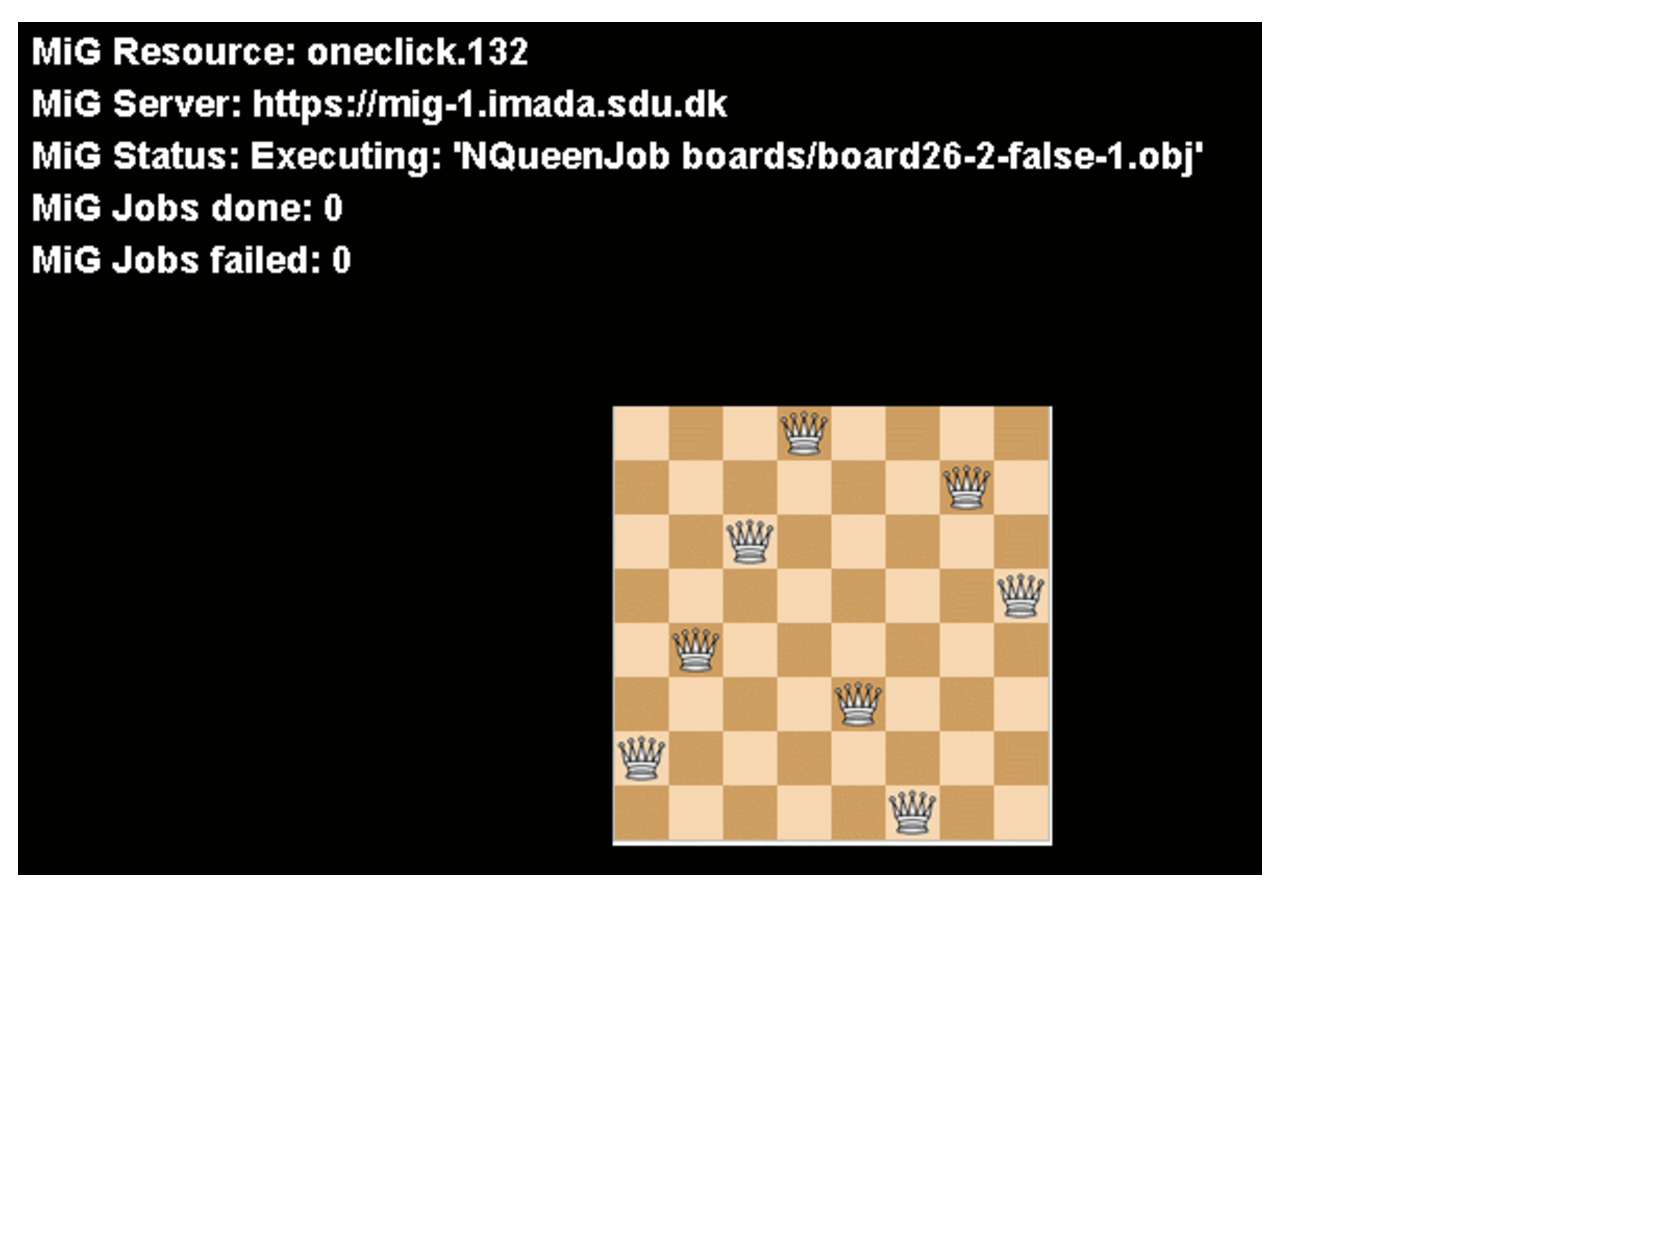
\includegraphics{actionshot.pdf}
\caption{\nq\ for 26 på \oc.}
\label{fig:action}
\end{figure}
\end{landscape}

%\subsection*{Problemformulering}
Opgavens formål er at implementere en parallel udgave af Takakens algoritme til løsning af n-dronning-problemet. Algoritmen skal køre på MiG-systemet (Minimum Intrusion Grid) og MiG's one-click arkitektur skal kunne udnyttes til at skaffe ressourcer til beregning af problemet. Formålet er på langt sigt at få beregnet en løsning til N-dronning-problemet for $n=26$, men opgaven er kun at gøre dette muligt ved hjælp af MiG. N-dronning-problemet er et klassisk beregningsproblem, der går ud på at finde antallet af mulige måder n dronninger kan placeres på et "skakbræt" med n x n felter, uden at nogen af dem er istand til at slå hinanden i næste træk. Problemets størrelse stiger eksponentielt med n, og er uhyre beregningstungt for store n, hvorfor store distribuerede systemer ofte benyttes. Hidtil er der kun fundet løsninger for $n \in \{1,...,25\}$. For distlab-gruppen her på diku ville en løsning for $n=26$, beregnet på et MiG-grid, kunne skabe opmærksomhed omkring MiG-systemet. 

MiG er beskrevet indgående i \cite{simplemig} og \cite{mig}, \cite{etsi} beskriver N-dronning-problemet grundigere end ovenstående og præsenterer en løsning for n=25. Appendix queens.c i \cite{etsi} er en udskrift af Takakens algoritme implementeret i C.
One-click muliggør deltagelse i et MiG-grid uden andre forudsætninger end en webbrowser og java. Tilgengæld er denne metode begrænset til at afvikle programmer, der er tilgængelige som java-bytecode. Brug af one-click giver adgang til et enormt (potentielt) antal beregningsressourcer, hvilket er grunden til at benytte one-click i denne opgave.    

Opgaven indeholder altså følgende delproblemer: 
\begin{itemize}
\item At finde en effektiv strategi til parallelisering af Takakens algoritme. Herunder overvejelser omkring den optimale størrelse på delproblemer.
\item Implementation af algoritmen i java på en sådan måde at den kan afvikles af one-click-klienter. 
\item Strategi for indsamling, behandling og præsentation af delresultater. 
\item Første opgave er naturligvis at få et bedre kendskab til MiG.
\end{itemize}

%Projektets form�l er ikke at beregne en l�sning til N-dronning-problemet for $n=26$, hvilket problemets beregningsm�ssige omfang kombineret med tids- og ressourcebegr�sninger udelukker i praksis. Men kun at muligg�re og forh�bentlig igangs�tte denne beregning. 
Vi vil ikke tage stilling til den benyttede algoritmes korrekthed eller effektivitet, men kun til den bedst mulige strategi for parallelisering. Partitionering af problemdata skal foreg� p� en fornuftig m�de, med tanke p� hvordan det forventes beregningsressourcerne opf�rer sig, men en decideret statisk unders�gelse af midlertidige MiG-ressourcers opf�rsel eller levetid vil ikke blive foretaget\footnote{Med ressourcers opf�rsel t�nkes p� den tid man kan forvente en bruger vil lade sin one-click-klient k�re}. Fordele og ulemper ved MiG eller One-click i forhold til andre grid-systemer falder ogs� udenfor opgavens omfang. 


%\landscape
\begin{multicols}{2}
\tiny
\section{Benchmark Output}
zomg.. benchoutput should be here.. 
\end{multicols}

%\begin{multicols}{2}[\section{\LaTeX kildekode}]
%\section*{Skabelon.tex}
%\verbatiminput{skabelon.tex}
%\end{multicols}

\end{document}
